\chapter{Retrieval, Grounded Generation and Agent Design}

\section*{Introduction}
\addcontentsline{toc}{section}{Introduction}

The knowledge graph holds the facts. This chapter describes the layer that turns a typed or spoken question into an answer drawn from it. Three problems have to be solved in sequence: working out which activity the user means, working out what they want to know about it, and saying it back in a way that reads naturally without becoming unfaithful in the process.

The third problem is where most of the design effort went, and it is the one that distinguishes this system from a conventional retrieval-augmented assistant. The language model here is not trusted to decide anything. It receives facts that have already been retrieved and is permitted only to rephrase them, and what it produces is verified against those facts before it is shown.

\section{Retrieval Methodology}

\subsection{Identifier Fast Path}

When a question contains something shaped like an activity identifier, the system tries a direct lookup first. Identifiers are unique, so a match is exact and carries no uncertainty. This path is cheap and it is the one that serves users who already know what they are looking for.

An identifier that is not in the node set is treated as a distinct outcome rather than as a failed lookup. This distinction matters more than it sounds. In an earlier version, an unrecognised identifier simply fell through to free-text search over the whole question, including the bogus identifier itself. The remaining words in the question, things like ``task'', ``who'', and ``approves'', share enough vocabulary with real activity titles to score above zero, so the system would return a confident answer about an unrelated activity while the user believed they were being told about the identifier they had asked about. The behaviour was reachable with ordinary phrasing, not a contrived edge case.

\subsection{Free-Text Resolution}

Questions that name an activity rather than identifying it are resolved by lexical similarity. Activity titles are vectorised with TF-IDF and compared against the question by cosine similarity, and the highest-scoring node is returned along with its score.

Process-level titles are included in the index alongside tasks, child tasks, and threshold variants. They were excluded at first, on the reasoning that users ask about activities rather than about organisational groupings. That reasoning was wrong in a specific way: a user asking about the organisation of missions in the non-sovereign chapter was matching nothing useful, because the only node whose title actually contained that phrasing was a process and processes were not indexed.

\subsection{Why Lexical Retrieval Rather Than Embeddings}

Semantic retrieval with learned embeddings is the more fashionable choice and would be the right one for a large, varied corpus written in ordinary language. This corpus is neither large nor varied. It is a few hundred short titles written in a controlled institutional vocabulary, where the words a user is likely to type are mostly the words the document already uses.

Lexical matching also has a property that matters for this project: its behaviour is explainable. A score can be traced to shared terms, a mismatch can be diagnosed by looking at the vocabulary, and the whole layer runs with no model download, no inference cost, and no dependency on an external service. Given that retrieval accuracy is the foundation everything else rests on, the ability to reason about why a given node was returned was worth more than the additional recall an embedding model might have offered.

\subsection{Typo Tolerance}

People misspell things, particularly long institutional phrases. Rather than relying on a language model to interpret intent, the system applies a deterministic correction step: each alphabetic word in the question is compared against the vocabulary the document itself uses, and replaced with the closest match when the similarity exceeds a threshold and the word is not already an exact match.

The threshold was calibrated against a real false positive rather than chosen by intuition. Set too low, ordinary words get rewritten into document vocabulary they merely resemble, which corrupts questions that were correct to begin with. Because the step is deterministic, it behaves identically whether or not a language model provider is reachable.

\section{Evaluation Protocol and Confidence Semantics}

There is no held-out test set here, because there is no labelled corpus to hold out. Correctness is established instead by comparison against the source document, and every resolution carries a method label and a confidence value so that the basis of an answer is visible to the user rather than implied.

\begin{longtable}{|p{0.26\textwidth}|p{0.18\textwidth}|p{0.46\textwidth}|}
\caption{Resolution methods and their confidence semantics.}\label{tab:methods}\\
\hline
\rowcolor{thesisgreen}\textcolor{white}{\textbf{Method}} & \textcolor{white}{\textbf{Confidence}} & \textcolor{white}{\textbf{Interpretation}} \\
\hline
\endfirsthead
\hline
\rowcolor{thesisgreen}\textcolor{white}{\textbf{Method}} & \textcolor{white}{\textbf{Confidence}} & \textcolor{white}{\textbf{Interpretation}} \\
\hline
\endhead
\texttt{id} & 1.0 & Exact identifier match. No ambiguity. \\ \hline
\texttt{text\_search} & TF-IDF score & Resolved from the activity's name. The score is shown, and low scores are flagged in the interface. \\ \hline
\texttt{invalid\_id} & --- & An identifier was recognised in the question but does not exist in the document. \\ \hline
\texttt{needs\_clarification} & --- & The question is too vague to resolve to a single activity. \\ \hline
\texttt{out\_of\_scope} & --- & The question is not about the subject matter of the document. \\ \hline
\texttt{glossary} & --- & The question asked for the expansion of an abbreviation. \\ \hline
\texttt{action\_code\_legend} & --- & The question asked what an authority code means. \\ \hline
\texttt{smalltalk} & --- & Conversational input with no lookup component. \\ \hline
\end{longtable}

Exposing the method alongside the answer is a small decision with a large effect on trust. A user who can see that an answer came from an exact identifier match treats it differently from one resolved by name at a middling similarity score, and that difference in treatment is appropriate.

\section{Deterministic Answer Construction}

\subsection{Intent Detection}

Once an activity is resolved, the system determines what is being asked about it. Questions map onto the document's authority codes, and the mapping has to accommodate the way people actually phrase things: ``who signs off on this'' means approval, ``who has to check this'' means check and verify.

The mapping is deliberately not naive about the letter C. As set out in Chapter~1, C1 and C2 mean check and verify while C3 and C4 mean consult, and treating the word ``check'' as equivalent to the bare letter C would merge two unrelated obligations. Intent detection therefore works against full codes rather than their first character.

\subsection{Mandatory Obligation Surfacing}

An answer reports what was asked and then adds what the document makes mandatory regardless. If an activity has a recorded check-and-verify obligation, that obligation is stated even when the question was about approval. If informed parties are recorded, they are named.

The reasoning is that these are not contextual extras. A check-and-verify entry in the DAM is an institutional requirement, and a new employee asking a narrow question is exactly the person who does not know to ask the other three. The note is suppressed only when it would duplicate the answer already given.

\subsection{Cross-Reference Following}

Where a resolved activity has no responsibilities of its own but does carry a cross-reference, the system follows the reference and reports the target's responsibilities, stating that it has done so. This mirrors what a human reader does when a row tells them to look elsewhere, and it converts a dead end into an answer.

\subsection{Honest Refusal}

Three cases produce an explicit non-answer. An identifier that does not exist is reported as not existing, with a suggestion to check it or describe the activity in words. A question too vague to resolve prompts for more detail. A question outside the document's subject matter is declined as out of scope.

None of these paths is allowed to degrade into a best guess. This is the behaviour that requirement FR7 specifies and the property that gives the system's positive answers their value: a tool that answers everything tells you nothing about which of its answers to trust.

\section{Auxiliary Query Types}

Not every question is an authority lookup. Three additional categories are handled directly.

Glossary questions ask what an abbreviation means and are answered from the abbreviations parsed out of the document, supplemented by a small curated set of aliases for acronyms that appear in role names without being separately defined. When an expansion comes from the curated set, the system says so rather than presenting it as sourced from the document.

Authority-code questions ask what a code means and are answered from the transcribed legend. Detection here is deliberately conservative about bare single letters, since ``I'' collides constantly with the pronoun. A bare code counts as a real mention only when it appears alongside another code or is unambiguous on its own, such as the parenthesised informed marker or a letter-and-digit combination that is not a plausible English word.

Conversational input, greetings and thanks and questions about what the system can do, is matched against anchored patterns and answered directly, short-circuiting the lookup pipeline. The patterns are anchored against the whole message rather than searched as substrings, because a substring test matches ``hi'' inside ``history of the DAM''.

\section{Hybrid Language Model Layer}

Answer phrasing is delegated to a language model through a provider interface with two implementations and four operating modes.

\begin{longtable}{|p{0.16\textwidth}|p{0.30\textwidth}|p{0.44\textwidth}|}
\caption{Language model providers and operating modes.}\label{tab:llm}\\
\hline
\rowcolor{thesisgreen}\textcolor{white}{\textbf{Mode}} & \textcolor{white}{\textbf{Provider}} & \textcolor{white}{\textbf{Behaviour}} \\
\hline
\endfirsthead
\hline
\rowcolor{thesisgreen}\textcolor{white}{\textbf{Mode}} & \textcolor{white}{\textbf{Provider}} & \textcolor{white}{\textbf{Behaviour}} \\
\hline
\endhead
Auto & Cloud, falling back to local, then template & Default. Uses whichever provider is available, and the deterministic template if neither is. \\ \hline
Cloud & Groq & Hosted inference. Fast, requires an API key and network access. \\ \hline
Local & Ollama & Runs on the same machine or in a companion container. No external dependency. \\ \hline
Off & None & Template answers only. Every lookup capability remains available. \\ \hline
\end{longtable}

The interface between the agent and the providers is narrow by design, which paid off during the project when a hosted model was deprecated by its provider and began returning errors on the deployed instance. The fix was a single constant change behind the interface, with no effect on the agent, the retrieval layer, or the tests covering them.

\section{Grounded Generation and the Verification Check}

\subsection{The Contract Given to the Model}

The model never sees the knowledge graph and never chooses what to retrieve. It receives a question, a set of already-retrieved facts, and a system prompt instructing it to state those facts naturally, to invent nothing, to omit nothing, and to avoid formatting of any kind. Where the answer must be produced in another language, an additional rule instructs it to translate the sentence while copying role names, identifiers, and footnote numbers exactly as given.

\begin{figure}[htbp]
\centering
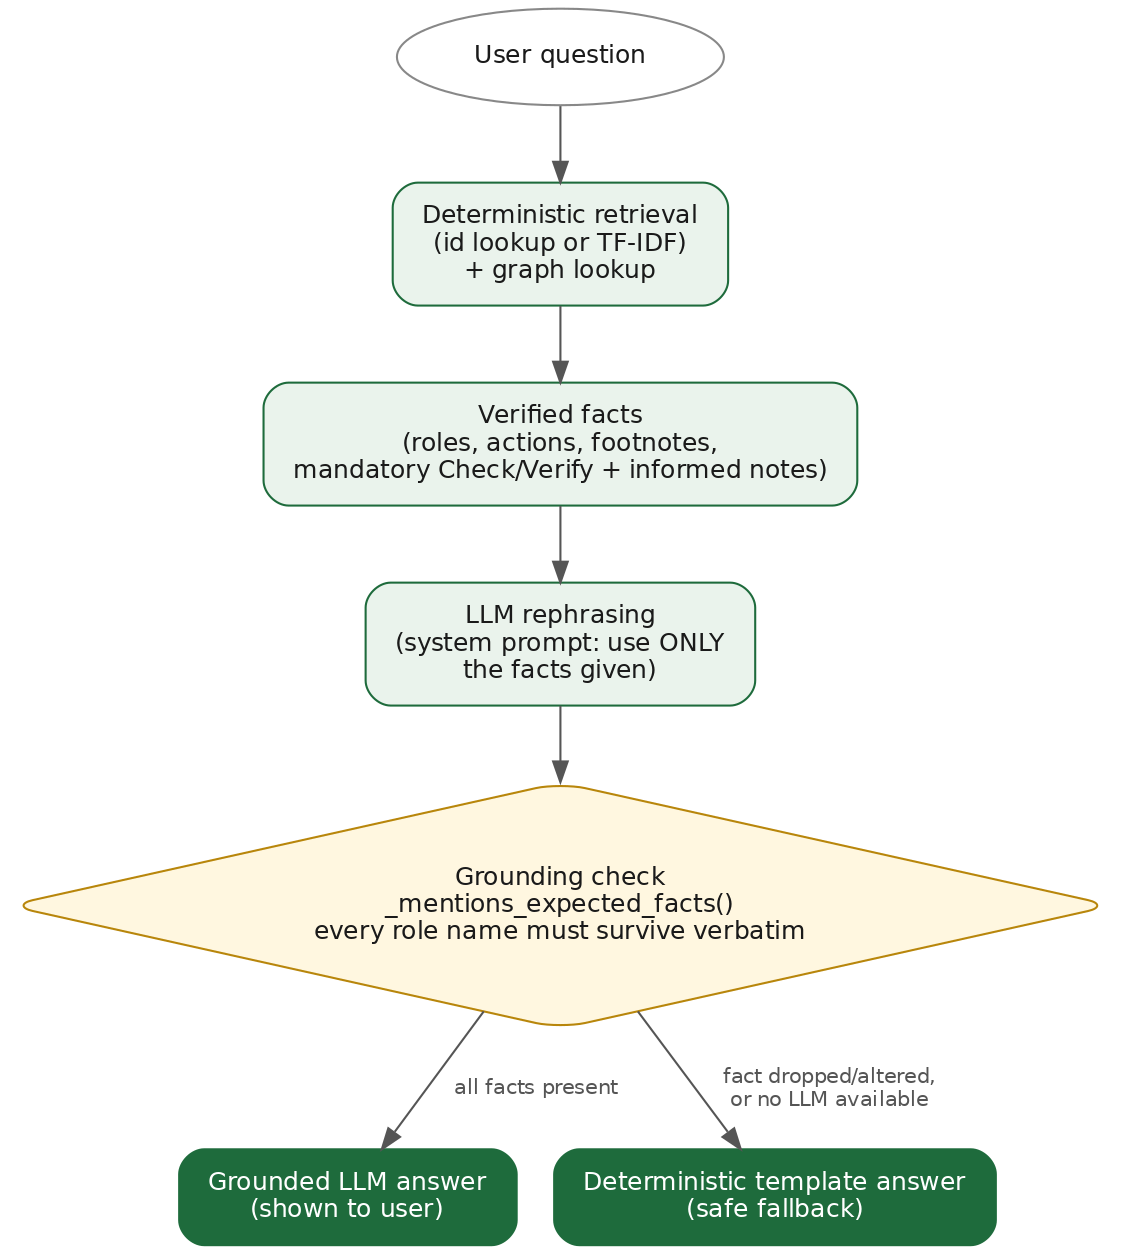
\includegraphics[width=0.82\textwidth,height=0.8\textheight,keepaspectratio]{figures/fig4_grounding.png}
\caption{The grounded generation flow. The model may only rephrase facts that have already been verified, and any rephrasing that drops or alters a fact is discarded in favour of the deterministic template answer.}
\label{fig:grounding}
\end{figure}

\subsection{The Verification Step}

A prompt is an instruction, not a guarantee. The verification step is what turns the instruction into a property of the system.

Before a generated answer is returned, every role name in the facts backing that answer is checked for presence in the generated text. If any is missing, the generated answer is discarded and the deterministic template answer is returned in its place. The check is a containment test rather than a similarity judgement, which means it cannot be satisfied by a paraphrase: a model that renames a role, merges two roles into one, or quietly drops the third of four informed parties fails the check, regardless of how fluent the result is.

Comparison is performed after normalising whitespace and case on both sides. That tolerance was added after the check was observed rejecting otherwise faithful rephrasings over nothing but incidental spacing differences. It loosens formatting sensitivity without loosening what is actually verified, since the same words in the same order must still be present.

\subsection{Answer Length and the Fallback Rate}

The verification step initially fired more often than expected, and the cause turned out to be a conflict between two instructions rather than model unreliability. The system prompt asked for an answer in one to three sentences. Activities with many recorded responsibilities cannot be stated completely in three sentences, so the model, following the brevity instruction, dropped facts, and the check correctly rejected the result.

The fix relaxed brevity rather than accuracy. When the number of facts backing an answer reaches a threshold, the brevity rule is replaced with an instruction to use as many sentences as the facts require, while every other constraint stays in place. The fallback rate dropped and the verification criterion was left untouched, which was the point: the accuracy requirement was never the thing that needed adjusting.

\section{Conversational Capabilities}

\subsection{Context Carry-Over}

A user who has just asked about an activity and then asks ``and who has to be informed?'' expects the second question to be understood against the first. The interface passes the previously resolved activity identifier with each question, and where a follow-up contains no subject of its own, it is answered against that activity, with the interface stating that the subject was carried over.

Carry-over is suppressed for question types that have nothing to do with the previous activity. Authority-code questions were briefly swallowed by it, so that asking what a code means while an activity was in context produced an answer about that activity instead of about the code.

\subsection{Tone Adaptation}

Questions are classified as neutral, frustrated, or confused, and a short empathetic opener is prepended where the tone is not neutral. Classification runs only when a cheap pre-filter suggests it is worth doing, so the common case costs nothing extra, and it is applied to what the user actually typed rather than to any internally translated version of it.

\subsection{Multilingual Questions}

Questions in French, Spanish, Portuguese, or Arabic are detected by a cheap pre-filter based on character ranges and function-word lists, translated into English for retrieval, and answered in the language they were asked in. Retrieval itself remains English-only, which keeps the index and its behaviour unchanged.

The verification check is not translated. It continues to look for the literal English role names inside the answer, whatever language the surrounding sentence is in, which is deliberate: a French answer that dropped a role name fails exactly as an English one would.

\section{Worked Examples}

The following exchanges were run against the delivered build and are reproduced as the system produced them.

Asking \textit{``who approves 2.126''} resolves by identifier with confidence 1.0 to the quarterly mission programme activity, and names the Regional Director General and the Director of the Nigeria office as approvers, with the abbreviation expanded inline. The answer also states that the task must be checked and verified by the Sector Manager and the Supporting Department Division Manager, and that the concerned Sector Vice-President, the Regional Vice-President, and the Task Manager or Project Team must be informed. None of that was asked for. All of it is mandatory.

Asking \textit{``who needs to be informed for quarterly mission program''} resolves the same activity from its name alone, with the answer now centred on the informed parties.

Asking \textit{``who aproves the qaurterly mision program''}, with two deliberate misspellings, resolves identically. The correction is deterministic, so it behaves the same with or without a model provider available.

Asking \textit{``who initiates 1.117.2''} exercises the redirect path. That activity's own row records no responsibilities and points to another activity, so the system follows the pointer and reports the target's responsibilities instead of dead-ending.

Asking \textit{``who approves of Communication with Co-Financiers of projects''} followed by \textit{``and who are the informed parties?''} exercises carry-over: the second question stays on the activity resolved by the first.

Asking \textit{``what happens with 9.999.999''} produces a refusal, stating that the identifier does not exist and suggesting the user check it or describe the activity in words. This is the behaviour the design exists to produce, and it is worth reading it as a result rather than as a limitation.

\section*{Conclusion}
\addcontentsline{toc}{section}{Conclusion}

The agent resolves questions through an identifier fast path and a lexical search layer, both deterministic, and constructs answers from records held in the graph. A language model improves how those answers read and is prevented from affecting what they say by a verification step that compares generated text against the retrieved facts and discards anything that has lost one. Around that core sit the behaviours that make the system usable in practice: typo tolerance, redirect following, mandatory obligation surfacing, context carry-over, multilingual handling, and explicit refusal. The next chapter presents the platform built on top of this agent.
